\documentclass[a4paper,12pt]{article}
\usepackage[utf8]{inputenc}
\usepackage[MeX]{polski}
\usepackage[table,xcdraw]{xcolor}
\usepackage[utf8]{inputenc}
\usepackage[T1]{fontenc}
\usepackage{graphicx}
\usepackage{epstopdf}
\usepackage{color}
\usepackage{mathtools}
\usepackage{pbox}
\usepackage{longtable}
\usepackage[hidelinks]{hyperref}
%%%%%%%%%%%%%%%%%%%%%%%%%%%%%%%%%%%%%%%%%%%%%%%%%%%%%%%%%%%%%STRONA TYTULOWA%%%%%%%%%%%%%%%%%%%%%%%%%%%%%%%%%%%%%%%%%%%%%%%%%%%%%%%%%%%%%%%%%%%%%%%%
\title{\Huge \textbf{Politechnika Wrocławska\\[0.3in]} 
  \huge SPD \\[0.2in]
  \LARGE Opracowanie
}
\date{}
	\author{
 	\quad	\\
}

\begin{document}
\maketitle
\pagebreak

\tableofcontents
\pagebreak

\section{Przykładowe zadania optymalizacji. Klasyfikacja podejść i metod}
	\subsection{Przykładowe zadania optymalizacji}
	\begin{itemize}
		\item Problem plecakowy - zadanie to polega na zapakowaniu do plecaka przedmiotów
		 tak, aby osiągnąć maksymalną sumaryczną wartość przedmiotów zapakowanych
		 przy ograniczonej pojemności plecaka.
		 \item Problem komiwojażera (TSP) - polega na znalezieniu minimalnego cyklu Hamiltona
		 w pełnym grafie ważonym. Odwzorowaniem tego problemu w rzeczywistości jest 
		 rozwiązanie problemu podróżnego handlarza, który chce odwiedzić wszystkie
		 zaplanowane miasta minimalizując jednoczenie drogę lub czas lub koszt odbycia tej
		 podróży.
		 \item Optymalizacja procesu wytwarzania - uszeregowanie zadań w taki sposób aby
		 zostało osiągnięte zadane kryterium np. minimalizacja czasu wykonania wszystkich
		 zadań.
	\end{itemize}
	\subsection{Klasyfikacja podejść i metod}
	\begin{enumerate}
		\item Metody dokładne
			\begin{itemize}
				\item Schemat podziału i ograniczeń (B\&B) - ogólne podejście oparte na dekompozycji
				(podziału na mniejsze problemy, redukcja ograniczeń) i
				"inteligentnym" przeszukiwaniu zbioru rozwiązań dopuszczalnych problemu optymalizacyjnego.
				Znajduje zastosowanie w problemach silnie NP-trudnych. Dostarcza algorytmów o wykładniczej
				złożoności obliczeniowej. Może być stosowany dla dowolnego problemu dyskretnego (liniowego i
				nieliniowego).
				\item Schemat programowania dynamicznego (PD) - podejście polegające na przekształceniu zadania
				optymalizacji w wieloetapowy proces podejmowania decyzji, w którym stan na każdym etapie
				zależy od decyzji wybieranej ze zbioru decyzji dopuszczalnych. Stany poprzednich etapów
				zostają zapamiętane zatem eliminowana jest konieczność kilkukrotnego przeliczania tych 
				samych rozwiązań (porozwiązywań). Złożoność algorytmów dla tego podejścia może być 
				wielomianowa(max droga w grafie), pseudowielomianowa(problem załadunku) 
				jak i wykładnicza(TSP).
				\item Programowanie liniowe całkowitoliczbowe (PLC) - podejście w którym zarówno funkcja celu 
				jak i zestaw ograniczeń składają się z funkcji liniowych z żądaniem aby wszystkie 
				parametry były wyrażone liczbami całkowitymi.
				\item Programowanie liniowe binarne (PLB) - tak jak PLC, w którym parametry przyjmują 
				wartości binarne (0,1).
				\item Metody subgradientowe - mogą byś stosowane dla przypadków, gdzie funkcja celu jest
				funkcją ciągłą i subróżniczkowalną, posiadającą skończoną wartość ekstremum, a zbiór 
				rozwiązań jest niepusty, domknięty i wypukły. Metody te s ą kosztowne obliczeniowo, a ich
				szybkość zbiegania do rozwiązania optymalnego silnie zależy od przykładu problemu.
			\end{itemize}
		\item Metody przybliżone - są to metody, które nie znajdują rozwiązania optymalnego, lecz
		rozwiązanie bliskie optymalnemu. Są stosowane tam, gdzie ważniejsze jest szybkie otrzymanie 
		rozwiązania.
			\begin{itemize}
				\item Konstrukcyjne - szybkie, łatwe w implementacji lecz rozwiązanie dość znacznie
				odbiega od rozwiązania optymalnego.
				\item Poprawiające - wolniejsze, wymagają podania początkowego rozwiązania rozwiązania,
				które poprawiają w kolejnych krokach. Dostarczają rozwiązań o bardzo dobrej i doskonałej
				jakości. Umożliwiają kształtowanie kompromisu pomiędzy jakością a czasem obliczeń.
			\end{itemize}
	\end{enumerate}
\section{Optymalizacja procesu wytwarzania. Szeregowanie.}
	\subsection{Optymalizacja procesu wytwarzania}
	
	Proces wytwarzania jest rozbudowanym zagadnieniem. W celu jego optymalizacji należy zwrócić uwagę na:
	\begin{itemize}
		\item synchronizację terminów dostaw z zapotrzebowaniami,
		\item odpowiednim przydzieleniu w czasie zasobów do wykonywanych zadań,
		\item podział zadań na partie produkcyjne,
		\item uszeregowanie zadań (określenie ich terminów wykonywania na poszczególnych maszynach)	
	\end{itemize}		
	
	\subsection{Szeregowanie}
	Szeregowanie zadań w procesie wytwarzania jest kluczowym elementem optymalizacji tego procesu.
	Na podstawie problemu praktycznego tworzony jest opis przy użyciu pojęć z teorii szeregowania, który
	prowadzi do matematycznego modelu procesu. Symboliczny opis problemu szeregowania:
	
	\begin{equation}
		\alpha|\beta|\gamma
	\end{equation}
	
	$\alpha$ - typ zagadnienia, \newline
	$\beta$ - dodatkowe ograniczenia, \newline
	$\gamma$ - postać funkcji celu. \newline
	
	W typie zagadnienia zawarte są informacje o ilości maszyn, sposobie przejścia zadań przez system 
	(typ zagadnienia: przepływowy, gniazdowy, równoległy) oraz o trybie realizacji poszczególnych operacji zadania. \newline
	Pośród przykładowych dodatkowych ograniczeń można wymienić takie jak: prec - narzucony, częściowy porządek 
	wykonywania zadań, pmtn - dopuszczenie możliwości przerwania wykonywania zadania, setup - wstępują czasy 
	przezbrojenia maszyn pomiędzy wykonywaniem zadań i inne.  \newline
	Przykładowa funkcja celu może być w postaci minimalizacji czasu wykonania wszystkich zadań. \newline
	
	Problem szeregowania zazwyczaj jest problemem NP-trudym. Istnieje wiele algorytmów dokładnych jak i przybliżonych
	rozwiązujących problemy tego typu.
	
\section{Strategie wytwarzania. Systemy sterowania}
\subsection{Systemy sterowania}
System sterowania ma zapewnic uruchamianie, nadzorowanie i zapewnienie realizacji zadan produkcyjnych. W zaleznosci od wielkosci produkcji, jej charakteru linii produkcyjnej i stoppnia automatyzacji parku maszynowego stosowane sa rozne strategie wytwarzania.

\subsection{Strategie wytwarzania}
\subsubsection{PUSH}
Zadania wytworcze (zamowienia na produkt koncowy) sa tlumaczone na zadania materialow i polproduktow a nastepnie przepychane przez system sterowania produkcj? wed?ug ustalonego harmonogramu. W razie potrzeby harmonogram jest na bierzaco korygowany i odpowiednie sterowania sa przekazywane do systemu wytwarzania. Sterowanie tego typu nosi nazwe nadaznego

Systemy sterowania dla tej strategii to MRP i ERP.
\begin{itemize}
\item MRP - Material Requirements planning -  Umozliwia kontrole rodzajow ilosci i terminow produkcji a takze sterowanie zapasami i ich uzupelnianiem
\item ERP - enterprise resource planning - system wspomagajacy nadzor nad calym procesem produkcji poczawszy od zaopatrzenia w materialy a skonczywszy na dostawie do odbiorcy.
\end{itemize}

Strategie polecana dla produkcji jednostkowej i krotkoseryjnej.
\subsubsection{SQUEEZE}
Strategia zak?ada ?e wydajnosc systemu wytworczego jest ograniczona przepustowoscia waskeigo gardla systemu. Gard?o to zestaw stanowisk wytworczych przez ktore produkcja sie przeciska powodujacspietrzanie i kolejki zadan.

Jeno jeden system OPT : 
umozliwia zoptymalizowanie przeyplywu produkcji koncentrujac sie na waskim gardle upatrujac w nim element determinujacy dzialanie calego systemu produkcyjnego.

Strategia polecana dla produkcji krotko i srednio seryjnej.
\subsubsection{PULL ( JIT)}
Strategia zaklada za podstawe produkcji zgloszona wielkosc zapotrzebowania na okreslony produkt koncowy ktory powoduje ssanie na wyjsciu systemu. Przeklada sie to na ssanie materialow i polproduktow. Brak ssania oznacza bezczynnosc systemu i stanowisk wytwarzania , zapobiega zbednemu wytwarzaniu redukuje zapasy. 

KANBAN TOYOTA zamowienia gotowe na czas, karteczki etc. to chyba wiemy

\subsubsection{Inne strategie}
\begin{enumerate}
\item CAW - steruje zleceniami w celu zapewnienia stalego sredniego obciazenia stanowisk. Dobra jak stale terminy dostaw , stabilne dostawy materialow, niezmienna zdolnosc produkcyjna
\item CRS - ciagle uzupelnianie stawnow materialowych. Dobra dla produkcji seryjnej i powtarzalnej przy stalym zapotrzebowaniu

\end{enumerate}
\section{Problem Pakowania. Sformułowanie, własności i metoda rozwiązania}

	\subsection{Sformułowanie}
		Danych jest $n$ obiektów, każdy o rozmiarze $w_i$. Dane są również opakowania o pojemności $W$.
		Należy tak rozmieścić obiekty w opakowaniach aby użyć jak najmniej opakowań przy założeniu nie przekraczania
		pojemności opakowań.
		
	\subsection{Własności}
		\begin{itemize}
			\item Należy do zagadnień grupowania elementów.
			\item Jest problemem NP-trundym optymalizacji kombinatorycznej.
		\end{itemize}
		
	\subsection{Metoda rozwiązania}
	\begin{enumerate}
		\item Algorytmy przybliżone
			\begin{itemize}
				\item First Fit Decreasing (nazwa mówi wszystko :) - rozwiązanie nie gorsze niż 22\% optymalnego
				\item Przeszukiwanie z nawrotami - bardzo dobre rezultaty.
				\item Specjalizowany algorytm genetyczny Falkenauera.
			\end{itemize}
	\end{enumerate}
\section{Problem komiwojazera. Sformulowanie, wlasnosci i metoda rozwiazywania}

\subsection{Sformulowanie}
Dane jest n miast, ktore komiwojazer musi odwiedzic, oraz odleglosci miedzy kazda para miast. Celem jest znalezienie najkrotszej drogi laczacej wszystkie miasta zaczynajacej i konczocej sie w okreslonym punkcie. Sprowadza sie to do budowy grafu gdzie wierzcholki to miasta a wagi krawedzi to odleglosci miedzy nimi.
\subsection{Wlasnosci}
\begin{itemize}
\item Z uwagi na to ze powstaly graf jest grafem pelnym to na pewno posiada przynajmniej jeden minimalny cykl Hamiltona ( problem zawsze ma rozwiazanie).
\item Zagadnianie nalezy do problemow NP-trudnych - duza zlozonosc obliczeniowa wraz ze wzrostem liczby miast (nie wiadomo czy mozna rozwiazac w czasie wielomianowym).
\end{itemize}


\subsection{Metody}
Do rozwiazywania tego rpoblemu stosuje sie metody przyblizone.
Za pomoca metod programowania dynamicznego istnieje algorytm 'Held-Karp algorithm' (Helda-Karpia :D ?) ktory umozliwia rozwiazanie problemu w czasie$ O(n^22^n)$
\\ Ale algorytmy dokladne wolno dzialaja i raczej stosuje sie przyblizone. Algorytm mrowkowy, Lin-Kernighan, NN ( nearest neighbour)

Algorytm 2-optymalny - W podejściu tym bazujemy na obserwacji, iż krzyżujące się połączenia między miastami są zawsze gorsze niż takie, które się nie krzyżują.
W algorytmie tym zatem sprawdza się wszystkie możliwe pary krawędzi i jeśli którakolwiek
zawiera krawędzie krzyżujące się, następuje takie przestawienie czterech miast na trasie, by
krzyżujące się krawędzie zostały zastąpione przez takie, które się nie krzyżują. Jednakże, brak
krzyżujących się krawędzi wcale nie gwarantuje optymalności rozwiązania i cały proces
przeważnie kończy się w minimum lokalnym. Aby „uciec” z tego minimum lokalnego
wprowadzić można losowe zaburzenia do aktualnie najlepszej trasy 


\section{Problem plecaka}

	\subsection{Sformułowanie}
		Danych jest $n$ przedmiotów, każdy o objętości(wadze) $w_i$ oraz cenie(wartości) $c_i$.
		Dany jest również plecak o pojemności $W$
		Należy zapakować do plecaka przedmioty tak, aby ich sumaryczna wartość była możliwie jak największa przy
		nie przekroczeniu objętości plecaka.
		
	\subsection{Własności}
		\begin{itemize}
			\item Problem jest NP-trudny.
			\item Występuje w postaci ciągłej jak i dyskretnej.
		\end{itemize}
	\subsection{Metoda rozwiązania} \label{knapsack}
		\begin{enumerate}
			\item Metody dokładne
			\begin{itemize}
				\item Przegląd zupełny - generuje wszystkie dopuszczalne rozwiązania i z nich wybiera optymalne $O(2^n)$.
				\item Programowanie dynamiczne - złożoność pseudowielomianowa. Dzieli zadanie na mniejsze - prostsze do 
				rozwiązania. Na początku przyjmuje, że plecak ma pojemność 1, następnie generuje optymalne rozwiązanie
				dla plecaka o takiej pojemności, zapamiętuje je i inkrementuje pojemność plecaka tym razem szukając 
				rozwiązania optymalnego korzysta z wcześniej znalezionego rozwiązania dla mniejszej objętości plecaka.
				Ten schemat jest powtarzany aż do osiągnięcia wymaganej pojemności plecaka wraz z rozwiązaniem optymalnym.
			\end{itemize}
			\item Metody przybliżone
			\begin{itemize}
				\item Algorytm zachłanny - polega na posortowaniu przedmiotów niemalejąco według stosunku ceny do wagi 
				$\frac{c_i}{w_i}$. Następnie iterując całą posortowaną kolekcję od pierwszego elementu
				 umieszcza kolejno w plecaku te przedmioty, które wraz z przedmiotami umieszczonymi wcześniej nie 
				 przekraczają pojemności plecaka aż do końca kolejki lub całkowitego zapełnienia plecaka. 
				 Złożoność algorytmu $O(n logn)$.
			\end{itemize}
		\end{enumerate}

\section{Optymalizacja pracy jednomaszynowego stanowiska krytycznego. Sformułownie, własności i metoda rozwiązania.}
\subsection{Sformułowanie}
Problem polega na znalezieniu optymalnego harmonogramu wykonywania zadan na maszynie mogacej wykonywac tylko jedno zadanie w danym czasie. Zadania są charakteryzowane poprzez termin dostepności, czas wykonywania na maszynia oraz czas dostarczenia. Czasami również dopuszcza się możliwość przerywania zadań.
\subsection{Własność}
\begin{itemize}
\item problem NP-trudny, w szczególnych przypadkach istnieją algorytmy wielomianowe
\item Istnieje wiele opisów (niekoniecznie jednoznacznych) tego problemu jednak $1|r_j,q_j|C_{max}$  jest najpopularniejszy ze względu na autosymetrie ( zamiana miejscami $r_j z q_j$ posiada tę samą optymalną permutacje).
\end{itemize}
\subsection{Metoda rozwiązania}
Istnieje wiele metod rozwiązujących ten problem tak dokladnych jak i przyblizonych. Jednym z nich jest algorytm 2-aproksymacyjny S. Algorytm zakłada, ze jezeli maszyna jest wolna oraz co najmniej jedno zadanie jest gotowe do wykonania, nalezy skierowac do wykonania zadanie najpilniejsze ( to z najdluzszym czasem dostarczenia ).
\section{Optymalizacja pracy linii wytwórczej (problem przepływowy).
Sformułowanie, właściwości
i metoda rozwiązywania.}

	\subsection{Sformułowanie}
		Zbiór zadań $J=(1,2,...,n)$ jest przeznaczony do wykonania w podanej kolejności na $M=(1,2,...,m)$ maszynach o ograniczonej jednostkowej przepustowości. Każde zadanie $j\in J$ składa się z ciągu operacji $(O_1j, ..., O_mj)$. Operacja $O_ij$ odpowiada nieprzerywalnemu wykonywaniu zadania $j$ na maszynie $i$ w czasie $p_ij$. Rozwiązaniem jest harmonogram pracy maszyn reprezentowany przez macierze terminów rozpoczęcia oraz zakończenia zadań spełniające powyższe ograniczenia. W praktyce rozwiącanie jest całkowicie określone przez jedną z macierzy, gdyż aby otrzymać drugą wystarczy dodać/odjąć czasy wykonywania zadań $p_ij$. 

		
	\subsection{Własności}
	Problemy przepływowe są NP-trudne (wyjąwszy niektóre szczególne przypdaki).
	Dzielą się na dwa rodzaje:
\begin{enumerate}
\item Ogólne - gdy kolejność wykonywania zadań na maszynie może być różna dla każdej maszyny
\item Permutacyjne - gdy wszystkie permutacje są takie same (taka sama kolejność wykonywania zadań na wszystkich maszynach)
\end{enumerate}
	Problem permutacyjny jest częściej analizowany, głównie z powodu znacznie mniejszej ilości rozwiązań ($n!$, podczas gdy $n!^m$ dla problemu ogólnego. Często błąd pomiędzy rozwiązaniami jest optymalnymi obu typów problemów jest nieznaczny, czasem nawet rozwiązanie optymalne problemu ogólnego leży w klasie rozwiązań permutacyjnych. Rozwiązania problemów permutacyjnych mogą być wykorzystywane jako rozwiązania początkowe w algorytmach przybliżonych dla problemów ogólnych.
	
		
	\subsection{Metoda rozwiązania}
	Algorytm NEH - oparty na technice wcięć, do tej pory najlepszy wśród konstrukcyjnych algorytmów przybliżonych dla problemu permutacyjnego. Składa się z n-krokowej fazy zasadniczej poprzedzonej fazą wstępną. Zadania są sortowane nierosnąco po sumie czasów wykonań na maszynach. W fazie zasadniczej, w $j$-tym kroku, do istniejącej aktualnie permutacji, dokładane jest $j$-te zadanie z kolejki zadań wcześniej posortowanych. Jest ono wstawiane we wszystkie możliwe miejsca w akutalnej permutacji, dostarczając $j$ nowych permutacji. Permutacja o najmniejszej wartości funkcji celu przyjmowana jest jako najlepsza w tym kroku i uznawana za aktualną. 
	Analogią działania jest pakowanie torby na wyjazd - najpierw pakujemy jeden lub kilka największych elemetów, po czym kolejne coraz mniejsze elementy metodą "dopychamy" metodą prób.
\section{Optymalizacja systemu opartego na przepływie zadań}
	\subsection{Sformułowanie}
		Dane są:
		\begin{itemize}
			\item zbiór zadań $J={1, ..., n}$,
			\item zbiór maszyn $M={1, ..., m}$,
			\item zbiór operacji $O={1, ..., o}$
		\end{itemize}				
		Zbiór operacji jest dekomponowany na podzbiory odpowiadające zadaniom. Zatem zadanie $j$ składa się 
		z sekwencji $o_j$ operacji, które powinny zostać wykonane w zadanej kolejności (zgodnie z kolejnością w podzbiorze 
		$o_j$). Ponadto każda operacja musi zostać wykonana na przypisanej do niej maszynie, a maszyna może wykonywać
		tylko jedną operację w danej chwili czasu. \newline
		Na rozwiązanie dopuszczalne składa się wektor czasów rozpoczęcia wszystkich operacji. Najczęstszą formą funkcji celu
		jest minimalizacja $C_{max}$ - terminu zakończenia wszystkich zadań.
		
	\subsection{Właściwości}
		\begin{itemize}
			\item Problem można modelować za pomocą acyklicznego grafu $G(W)$, ($W$ - kompletna reprezentacja dopuszczalna).
			\item Problem jest NP-trudny.
		\end{itemize}			
	
	\subsection{Metoda rozwiązania}
		Jedną z metod rozwiązania problemu gniazdowego jest skorzystanie z algorytmu aproksymacyjnego.
		Nie generuje on rozwiązania optymalnego, jednakże jest bardzo wydajny obliczeniowo.
		Podstawowy algorytm aproksymacyjny składa się  z trzech kroków:
		\begin{enumerate}
			\item Wygeneruj rozwiązanie $S$ spełniające tylko wymagania porządku technologicznego tzn. zachowującego
			odpowiednią kolejność wykonywania operacji dla każdego zadania. Rozwiązanie takie jest niedopuszczalne, gdyż
			więcej niż jedno zadanie może zostać przydzielone do maszyny w tym samym momencie czas.
			W tym wypadku $C_{max}$ (dolne ograniczenie problemu gniazdowego) przyjmuje wartość $LB_J$ (suma czasów 
			wykonania najdłuższego zadania).
			\item Zaburz terminy rozpoczęcia operacji każdego zadania $i$ o wielkość $\delta_i$. Gdzie $\delta_i$
			jest całkowitą liczbą losową z rozkładu równomiernego na przedziale $[0, LB_M]$, gdzie $LB_M$ to suma czasów
			operacji na najbardziej "zajętej" (pracującej najdłużej) maszynie.
			\item “Rozciągnij” i “spłaszcz” otrzymane uszeregowanie tak, by w każdym
			momencie czasu na każdej maszynie było wykonywane nie więcej niż
			jedno zadanie.
		\end{enumerate}
		
		Inne metody służące do rozwiązania problemu gniazdowego:
		\begin{itemize}
			\item Schemat $B\&B$
			\item Algorytmy priorytetowe
			\item Przeszukiwania lokalne
			\item Metoda przesuwnego wąskiego gardła
			\item Symulowane wyżarzanie
			\item Poszukiwanie z zakazami
			\item Spełnianie ograniczeń
			\item Poszukiwanie ewolucyjne
			\item Podejście dualne
			\item Sieci neuronowe
		\end{itemize}

\section{Optymalizacja magazynowania. Przykładowy problem i metoda
rozwiązywania}
\subsection{Przykładowy problem}

Optymalizacja Procesów Magazynowych dotyczy czynności związanych z przyjmowaniem, składowaniem, kompletacją oraz wysyłką towarów w magazynach dowolnego typu (w tym wysokiego składowania). Pozwala na znalezienie oraz wyeliminowanie istniejących tzw. „wąskich gardeł”, określenie wymaganej wielkości poszczególnych stref obsługujących procesy magazynowe (w tym m.in. wielkość buforów na wejściu i na wyjściu z magazynu, centrum logistycznego, terminalu przeładunkowego czy innych obiektów infrastruktury logistycznej), określenie wymagań co do technologii zastosowanej w przypadku każdego z procesów magazynowych i wymaganej infrastruktury magazynowej. Może być zastosowane także w trakcie projektowania nowego magazynu w celu empirycznego określenia możliwych granic przepustowości magazynu jeszcze przed akceptacją jego projektu. Pozwala to na określenie niezbędnych do obsługi zasobów technicznych, w tym także do określenia optymalnego stopnia mechanizacji i automatyzacji procesów magazynowych.
Optymalizacja Procesów Magazynowych pozwala na:
\begin{itemize}
\item zwiększenie elastyczności procesów magazynowych
\item przyspieszenie przepływów towarów
\item eliminację lub redukcję problemu „wąskich gardeł”
\item skrócenie czasu przejścia towaru przez system logistyczny
\item obniżenie kosztów obsługi procesów magazynowych
\item optymalizację stref wykorzystywanych w przypadku realizacji poszczególnych procesów magazynowych
\item podniesienie poziomu obsługi
\end{itemize}

\subsection{Metoda rozwiązania}
Optymalizacja magazynowania wiąże się z identyfikacją kosztów utrzymania magazynu i ich częściowym obniżeniem bez uszczerbku na jakości wykorzystywanych materiałów eksploatacyjnych czy zagrożenia dla bezpieczeństwa pracy.
\subsubsection{Optymalizacja czasu pracy}
Na miejscu pracy powinna się znajdować optymalna liczba pracowników – niezbędna do realizacji wszystkich zadań.
\subsubsection{Obniżenie rachunków za energię elektryczną}
Koszty prądu w magazynach są znaczące. Można je jednak obniżyć, negocjując indywidualną stawkę z dostawcą energii. Warto rozmawiać nie tylko z dominującymi podmiotami, lecz także z mniejszymi dostawcami energii elektrycznej. Często ci mniejsi mają konkurencyjne oferty gwarantujące np. stałą cenę prądu na kilka lat. Gwarancja taka daje pewność, że koszty energii nie wzrosną, nawet gdy dojdzie do zmiany przepisów w prawie energetycznym.
\subsubsection{Zarządzania paletami}
Używanie przez magazyn drewnianych palet jest dla każdego przedsiębiorstwa kosztowne. Nie chodzi wyłącznie o ich zakup czy magazynowanie, lecz także o koszty transportu. Drewniane, ciężkie i wysokie palety można zastąpić tekturowymi, które przez to, że mogą być niższe, pozwalają załadować do samochodu ciężarowego więcej towaru. Dodatkowo są one lżejsze, co nie jest bez znaczenia dla kosztów paliwa. Koszty transportu spadają również z jeszcze jednego powodu. Papierowe palety są biodegradowalne i można je zostawić u klienta wraz z towarem. Zaleta tego rozwiązania jest taka, że zamiast wracać samochodem załadowanym wyłącznie paletami bez towaru, przed wysłaniem w drogę powrotną można go ponownie zatowarować.
\subsubsection{System identyfikacji pozycji magazynowej}
Im większy magazyn, tym trudniejsze jest znalezienie w nim np. małych partii produktów. Ważne jest, by pracownicy magazynu mieli możliwość natychmiastowego namierzenia poszczególnych produktów, a także identyfikacji poszczególnych pozycji. System automatycznej identyfikacji pozycji ułatwia pracę, jednak jest również wymagający – należy pamiętać o dokładnym wprowadzeniu produktu do systemu przy jego przyjęciu oraz o informowaniu o każdym jego późniejszym ruchu. Za pomocą tego systemu można w pełni automatycznie optymalizować alokację obiektów na regałach, co powoduje znaczące oszczędności w wykorzystaniu powierzchni magazynowej, a także czasu.
\subsubsection{Nowoczesny system IT}
Każdy nieplanowany przestój linii produkcyjnej generuje ogromne straty dla przedsiębiorstwa. Kosztochłonne są również zbyt wysokie stany zapasów (znaczące koszty magazynowania) oraz braki w magazynie. Dbanie o stany magazynowe jest ważne, gdyż umowy z kontrahentami obejmują wysokie kary za nieterminowe dostawy towarów. Można jednak nad tym zapanować, zlecając specjalistycznej firmie IT stworzenie dedykowanego systemu informatycznego, który będzie informował szefów działów (np. magazynu, zaopatrzenia) o brakach lub o stanach magazynowych. System taki może w znaczący sposób usprawnić pracę całego przedsiębiorstwa.
\section{Optymalizacja pracy linii wytwórczej (problem przepływowy).
Sformułowanie, właściwości
i metoda rozwiązywania.}

	\subsection{Sformułowanie}
		Zbiór zadań $J=(1,2,...,n)$ jest przeznaczony do wykonania w podanej kolejności na $M=(1,2,...,m)$ maszynach o ograniczonej jednostkowej przepustowości. Każde zadanie $j\in J$ składa się z ciągu operacji $(O_1j, ..., O_mj)$. Operacja $O_ij$ odpowiada nieprzerywalnemu wykonywaniu zadania $j$ na maszynie $i$ w czasie $p_ij$. Rozwiązaniem jest harmonogram pracy maszyn reprezentowany przez macierze terminów rozpoczęcia oraz zakończenia zadań spełniające powyższe ograniczenia. W praktyce rozwiącanie jest całkowicie określone przez jedną z macierzy, gdyż aby otrzymać drugą wystarczy dodać/odjąć czasy wykonywania zadań $p_ij$. 

		
	\subsection{Własności}
	Problemy przepływowe są NP-trudne (wyjąwszy niektóre szczególne przypdaki).
	Dzielą się na dwa rodzaje:
\begin{enumerate}
\item Ogólne - gdy kolejność wykonywania zadań na maszynie może być różna dla każdej maszyny
\item Permutacyjne - gdy wszystkie permutacje są takie same (taka sama kolejność wykonywania zadań na wszystkich maszynach)
\end{enumerate}
	Problem permutacyjny jest częściej analizowany, głównie z powodu znacznie mniejszej ilości rozwiązań ($n!$, podczas gdy $n!^m$ dla problemu ogólnego. Często błąd pomiędzy rozwiązaniami jest optymalnymi obu typów problemów jest nieznaczny, czasem nawet rozwiązanie optymalne problemu ogólnego leży w klasie rozwiązań permutacyjnych. Rozwiązania problemów permutacyjnych mogą być wykorzystywane jako rozwiązania początkowe w algorytmach przybliżonych dla problemów ogólnych.
	
		
	\subsection{Metoda rozwiązania}
	Algorytm NEH - oparty na technice wcięć, do tej pory najlepszy wśród konstrukcyjnych algorytmów przybliżonych dla problemu permutacyjnego. Składa się z n-krokowej fazy zasadniczej poprzedzonej fazą wstępną. Zadania są sortowane nierosnąco po sumie czasów wykonań na maszynach. W fazie zasadniczej, w $j$-tym kroku, do istniejącej aktualnie permutacji, dokładane jest $j$-te zadanie z kolejki zadań wcześniej posortowanych. Jest ono wstawiane we wszystkie możliwe miejsca w akutalnej permutacji, dostarczając $j$ nowych permutacji. Permutacja o najmniejszej wartości funkcji celu przyjmowana jest jako najlepsza w tym kroku i uznawana za aktualną. 
	Analogią działania jest pakowanie torby na wyjazd - najpierw pakujemy jeden lub kilka największych elemetów, po czym kolejne coraz mniejsze elementy metodą "dopychamy" metodą prób.
\section{Modele grafowe w badanich operacyjnych. Przykładowy problem i metoda rozwiazywania.}
http://www.thebookshelf.auckland.ac.nz/docs/NZOperationalResearch/1982vol10/Number1/ORSNZ-1982-10-1-04.pdf
\subsection{Problem}
dyscyplina naukowa związana z teorią decyzji pozwalająca wyznaczyć metodę i rozwiązanie określonych problemów związanych z podjęciem optymalnych decyzji. Obejmuje min. programowanie matematyczne , zagadnienie trapsortowe , zarzadzanie projektem teorie zapasow i kolejek.

Przykladem problemu moze byc metoda CPM, Innym moze byc problem komiowjazera, porlbem plecakowy, marszrutyacji w zasadzie cokolwiek
\subsection{Rozwiązanie}
Nie wiem :( , może bardziej chodzi o jakieś modele w stylu Activity on Node/Arrow a drzewa binarne / decyzyjne , zwykle grafy etc. a moze Macierz sasiedztwa lita sasiedztwa itp ? :D 


\section{Modelowanie dodatkowych ograniczeń w problemach planowania}

	W praktyce obok problemów przepływowych odpowiadających modelom
	podstawowym pojawiają się problemy bardziej
	złożone. Najczęściej są one pochodnymi zagadnienia podstawowego otrzymanymi
	poprzez wprowadzenie dodatkowych ograniczeń o różnym charakterze.
	
	\subsection{Transport}
	Przemieszczenie zadania pomiędzy maszynami w wielu przypadkach praktycznych jest tak duża, że modeluje się je jako
	maszynę o nieograniczonej przepustowości. Co zwiększa jednak niepotrzebnie rozmiar modelu grafowego.
	Aby tego uniknąć wystarczy dodatkowo obciążyć krawędzie grafu łączące operacje wykonywane na różnych maszynach
	czasami transportów pomiędzy tymi maszynami.
	\subsection{Przezbrojenia}
	Przezbrojeniem nazywamy czas potrzebny na zmianę oprzyrządowania
	maszyny w związku z wykonywanym zadaniem. Najbardziej ogólny przypadek
	zakłada, że czas ten zależy od maszyny oraz pary kolejno realizowanych
	po sobie zadań.
	\subsection{Stanowska o nieograniczonej przepustowości}
	Maszyna ma przepustowość $k$ jeżeli w dowolnym momencie może wykonywać nie więcej niż $k$ operacji równocześnie.
	Zatem za maszynę o nieograniczonej przepustowości można uważać:
	\begin{itemize}
		\item urządzenie, które w sensie fizycznym pozwala obsługiwać jednocześnie
		dowolnie wiele zadań, np. piec grzewczy,
		\item maszynę o ograniczonej przepustowości, dla której czas trwania jest
		nieporównywalnie mały w stosunku do maszyn sąsiednich przez co nie
		obserwuje się występowania kolejki,
		\item zbiór urządzeń fizycznych, identycznych funkcjonalnie i o tak dużej
		liczności, że operacje realizowane na tych urządzeniach nie muszą być szeregowane,
		\item maszynę otrzymaną poprzez zagregowanie (połączenie) podzbioru kolejnych
		maszyn o nieograniczonej przepustowości,
		\item maszynę fikcyjna realizującą proces wymagający upływu czasu lecz nie
		angażujący urządzenia w sensie fizycznym (operacje starzenia, schnięcia,
		dojrzewania, chłodzenia, itp.).
	\end{itemize}
	Termin gotowości zadania możemy interpretować jako wykonanie fikcyjnej operacji zadania na maszynie o 
	nieograniczonej przepustowości. \newline
	Problemy zawierające maszyny o nieograniczonej przepustowości zachowują
	swoje własności związane ze ścieżką krytyczną w grafie oraz własności eliminacyjne dotyczące bloków zadań.
	\subsection{Terminy dostępności}
	Termin dostępności zadania możemy modelować jako wykonanie fikcyjnej operacji zadania na maszynie o 
	nieograniczonej przepustowości.
	
	\subsection{Bufory}
	Bufor jest miejscem do chwilowego składowania zadania przekazywanego
	pomiędzy maszynami i jest zwykle związany z maszyną (bufor do maszyny).
	W obszarze bufora tworzona jest kolejka zadań do obsługi. Pojemność
	bufora jest rozumiana jako maksymalna liczba zadań, które mogą być składowane
	równocześnie. Klasyczne problemy szeregowania przyjmują zwykle,
	że pojemność bufora jest dowolnie duża (nieograniczona). Zadania, które po
	zakończeniu wykonywania na maszynie nie mogą być przekazane do odpowiedniego
	bufora pozostają na niej powodując zablokowanie tak długo aż
	pojawi się wolne miejsce w buforze. Logiczne pojęcie bufora może modelować:
	\begin{itemize}
		\item fizyczne urządzenie procesu technologicznego,
		\item ograniczony fizycznie obszar składowania,
		\item fikcyjne wymaganie “wymuszajace” przepływ produkcji.
	\end{itemize}
	Generalnie, rozpatrywane są dwie kategorie problemów: (1) z buforem o
	zerowej pojemności (ograniczenie no store, strategia NS), (2) z buforami o
	skończonej, ograniczonej pojemności, różnej dla różnych maszyn (strategia
	LS).
	
	\subsection{Czas cyklu}
	Jest to ograniczenie, które zakłada cykliczność produkcji zatem maksymalny czas wykonania wszystkich zadań
	jest ograniczony czasem cyklu. Gdy nie ma możliwości realizacji wszystkich zadań w jednym cyklu należy rozdzielić 
	je na kilka cykli.
\section{Modele harmonogramowania z dyskretnym czasem. Problem z jednym stanowiskiem obsługi}
Harmonogramowanie produkcji: rozłożenie w czasie przydziału zasobów do zleceń produkcji, podzielenie zadań na partię produkcyjne, określenie terminów rozpoczęcia i zakończenia realizacji partii na poszczególnych maszynach. Kompromis pomiędzy: kosztami niedotrzymania terminów, zaspokojeniem zapotrzebowania, kosztami utrzymania zapasów i zmian produkcji. 
Koszta zmiany produkcji wiążą się z przestojem maszyn, gdyż zachodzi potrzeba ich przezbrojenia.
W przypadku jednego stanowiska obsługi problem jest o tyle trudny, że nie można wykonywać dwóch typów zadań
bez przestoju. Istnieją dwa rodzaje podejść:
\begin{enumerate}
	\item Długi cykl i mała liczba przezbrojeń - w tym podejściu cykl trwa długo zatem produkowana jest znaczna ilość
	półproduktów co wymaga dużych zasobów magazynowych, jednakże w dłuższym okresie czasu minimalizuje liczbę przestojów 
	związanych z przezbrajaniem stanowiska. Produkty są wypuszczane rzadko w dużych ilościach.
	\item Krótki cykl i duża liczba przezbrojeń - cykl jest możliwie krótki dzięki czemu nie jest konieczna duża przestrzeń
	magazynowa i następuje cykliczne wypuszczanie małych serii produktów. Jednakże w dłuższym okresie czasu liczba 
	przestojów jest znaczna.
\end{enumerate}


\section{Schemat podziału i ograniczeń}
	\subsection{Charakterystyka metody}

		$B\&B$ nie określa żadnego konkretnego
		algorytmu lecz ogólne podejście oparte na dekompozycji (podziału na mniejsze problemy,
		relaksacji) i “inteligentnym”
		przeszukiwaniu zbioru rozwiązań dopuszczalnych problemu optymalizacyjnego.	
		Należy do metod dokładnych co implikuje znajdowanie rozwiązania optymalnego.
		Jego zastosowanie jest całkowicie uzasadnione tylko wtedy gdy uzyskamy pewność,
		że rozważany problem jest silnie NP-trudny. Schemat $B\&B$ dostarcza
		algorytmów o wykładniczej złożoności obliczeniowej.
		Może być stosowany dla dowolnego
		problemu dyskretnego z nieliniową badź liniową funkcją celu i takimi
		też ograniczeniami.
		Algorytmy te wymagają jednoznacznego określenia:
		\begin{itemize}
			\item reguły wyboru podzbiorów w których kolejno poszukiwane jest rozwiązanie,
			\item przyjętej relaksacji dostarczającej dolne organicznie,
			\item reguły eliminacji (odrzucania zbiorów w których nie ma oczekiwanych rozwiązań)
			\item zasady podziału podzbiorów,
			\item techniki dostarczającej górne ograniczenie
		\end{itemize}
		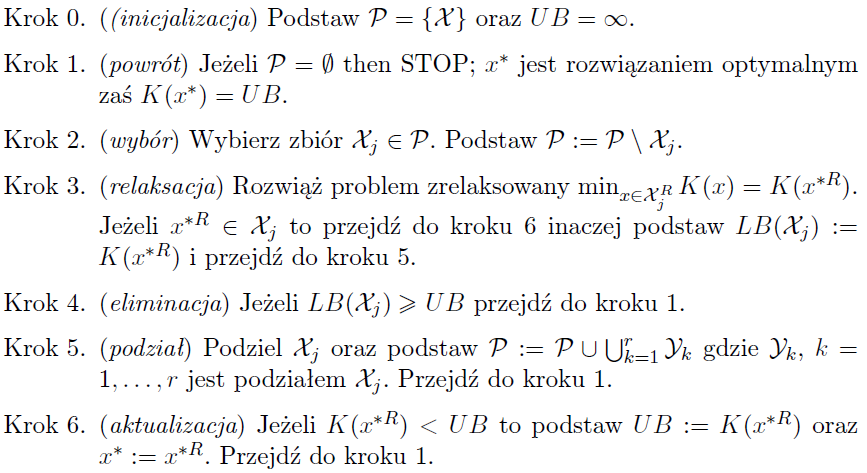
\includegraphics[width=1\textwidth]{alg.png}
	
	\subsection{Przykładowe zastosowanie}
		
		Przykładowym zastosowaniem tego schematu jest szeregowanie zadań w jedno maszynowym
		problemie z czasem dostępności, dostarczenia i możliwością przerwania zadań.
		Schemat ten implementuje algorytm Carliera, który do rozwiązywania problemów 
		zrelaksowanych wykorzystuje algorytm Schrage z podziałem.
\section{Programowanie dynamiczne}
	\subsection{Charakterystyka metody}

		Schemat ten określa ogólne podejście polegające na przekształceniu zadania
		optymalizacji w wieloetapowy proces podejmowania decyzji, w którym
		stan na każdym etapie zależy od decyzji wybieranej ze zbioru decyzji dopuszczalnych.
		Stany poprzednich etapów
		zostają zapamiętane zatem eliminowana jest konieczność kilkukrotnego przeliczania tych 
		samych rozwiązań (porozwiązywań). Złożoność algorytmów dla tego podejścia może być 
		wielomianowa(max droga w grafie), pseudowielomianowa(problem załadunku) 
		jak i wykładnicza(TSP).
		Jest to oczywiście metoda generująca rozwiązanie optymalne problemu.
		
	\subsection{Przykładowe zastosowanie}
	
		Programowanie dynamiczne znajduje zastosowanie w popularnym problemie plecakowym 
		(patrz \ref{knapsack}).
		
\section{Przyblizone metody rozwiazywania zadan optymalizacji. Miary i metody oceny}

\subsection{Tak ogolnie}}
Przyblizone metody rozwiazywania zadan optymalizacji wyznaczaja takie rozwiazanie ktore jest blisko rozwiazania optymalnego. Z uwagi na to ze poruszane problemy sa zazwyczaj NP-trudne to nie dziwi ze takich metod jest wiecej.
Miary oceny "dobroci" metody:
\begin{enumerate}
\item  zlozonosc obliczeniowa algorytmu
\item dokladnosc przyblizenia
\item gwarancja zbieznosci do rozwiazania optymalnego
\item szybkosc zbieznosci do rozwiazania optymalnego
\end{enumerate}

\\ Blad przyblizenia algorytmu mozna liczyc na wiele roznych sposobow np tak:
$BLAD = r. optymalne - r.otrzymane $\\
$BLAD = r. optymalne /r.otrzymane $\\
$BLAD = r. \frac{(r.optymalne - r.otrzymane)}{r.optymalne} $\\
$BLAD = r. \frac{(r.optymalne - r.otrzymane)}{r.otrzymane} $\\


Blad moze byc badany experymentalnie i teoretycznie - experyment najczesciej bo latwo, ale jest to subiektywne bo zalezy od probki przykladow. Dopiero wyniki analizy teoretycznej ( najgorsze przypadki etc.) w polaczeniu z wynikami analizy experymentalnej oraz zlozonosci obliczeniowej stanowia kompletna charakterystyke algorytmu.
\\

\subsection{Analiza experymentalna}
Najpopularniejsza, niedokladna. Ocena a posteriori zachowania sie algorytmu (blad przyblizenia, czas pracy) w oparciu o wynik przebiegu na nieprecyzyjnej acz reprezentatywnej probce. Otrzymane wyniki nie zawsze dostatecznie dobrze odzwieciedlaja wlasnosci numeryczne algorytmu, gdyz nie zawsze do konca wiadomo co oznacza pojecie probki reprezentatywnej
\subsection{Analiza najgorszegoprzypadku}
Analiza najgorszego przypadku ocenia a priori zachowanie sie wybranego bledu na calej populacji przykladow. Wyznacza sie wspolczynnik najgorszego przypadku i asymptotyczny wspolczynnik najgorszego przypadku (trudne wzorki).  Taka analiza dostarcza skrajnie pesymistycznych wnioskow, nie jest powiedziane ze w praktyce taka sytuacja kiedokolwiek wystapi.

\subsection{Analiza probabilistyczna}
Analiza aprioryczna, zaklada ze kazdy przyklad zostal otrzymany jako realizacja pewnej niezaleznej zmiennej losowej o znanym rozkladzie ( najczesciej rown. ). W takim podejsciu blad przyblizenia rowniez jest zmienna losowa. Przy tych badaniach wnioskuje sie o jego rozkladach momentach a co najwazniejsze zbieznosci do jakiejs wartosci stalej wraz ze wzrostem liczby probek oraz o szybkosci tej zbieznosci. Bardzo skomplikowana analiza, dostarcza niezlych wynikow jednak malo algorytmow ma takie opracowanie bo trudno sie to robi.


\end{document}

